\subsection{Performance Evaluation}\label{sec:cloud:data_centers:performance_evaluation}
Based on the metrics obtained in \refsec{sec:cloud:data_centers:modeling}, we can now compare the introduced default data centre and energy-efficient data centre models.

An optimal system setting would decrease both, waiting time and power drain.
For the discussion of this optimisation problem, we require additional notation which is introduced first.
We assume that the job inter-arrival rate \(\lambda\), the job service rate \(\mu\), and the total number of servers \(n_\text{total}\) are constants and not subject to the optimisation process.
Thus, the complete system can be described by the number of base-line servers \(n\), the server activation threshold \(\theta_2\), and the server deactivation threshold \(\theta_1\).
The number of reserved servers \(m\) can be easily derived if the total number of servers \(n_\text{total}\) is known.
Given these parameters, we define \(e(n, \theta_1, \theta_2)\) to be the mean power drain of the system and \(w(n, \theta_1, \theta_2)\) be the mean waiting time of all jobs.

%TODO: In die Introduction, also chap 0 ziehen?
A general approach for solving such multi objective optimisation problems is defining a single aggregate objective function, such as:
\begin{equation}
f(n, \theta_1, \theta_2) = \alpha e(n, \theta_1, \theta_2)  + (1-\alpha) w(n, \theta_1, \theta_2),
\end{equation}
for \(0\leq\alpha\leq 1\).
Then, it is possible to choose an \(\alpha\) in such a way that a desirable tradeoff is made. Thus, the optimisation problem can be defined as
\begin{align}
\min f(n, \theta_1, \theta_2) \qquad&s.t.& 1 < n < s,\\ 
&&1 < \theta_1 < n - 1,\nonumber\\
&&1 < \theta_2 < m - 1\nonumber,
\end{align}
and trivially solved by evaluating all valid parameter combinations, sorting the objective function values and choosing the minimum.

This approach has the obvious disadvantage that while a parameter combination may be optimal according to the chosen objective function, it may very well not be optimal to the stakeholders in the scenario.
For example, it may be possible that another system configuration exists with a minimally greater mean waiting time and a greatly reduced power drain.
To be able to decide whether such a tradeoff exists, a more global view of the problem space is required.
However, due to the number of possible parameter combinations, it is difficult to select appropriate parameters.
Thus, we reduce the number of possible parameters by considering only Pareto optimal states.

To define Pareto optimality, we need to introduce the product order partial relation. Let \(X\subseteq \mathbb{R}^n\) be our feature set.
We set \(x\preceq x^*\) for \(x, x^*\in\mathbb{R}^n\) iff
\begin{equation}
x_i \leq x^*_i \qquad\forall 1\leq i\leq n\\
\end{equation}
holds.
Then, \(x^*\) is Pareto optimal in \(X\) if no \(x\in X\backslash \left\{x^*\right\}\) exists, such that \(x\preceq x^*\) holds.

To study the system behaviour we consider an exemplary rack of \(n_\text{total} = 100\) servers, where new jobs arrive with a negative exponential inter-arrival time with mean \SI{10}{\milli\second}, yielding \(\lambda = \SI{1/10}{\per\milli\second}\).
To determine the mean service time we turn to \cite{Barroso07} where it is reported that in average servers are operating at \SIrange{10}{50}{\percent} of their maximum utilisation levels.
With this in mind we assume that the service time for job completion is again negative exponential with a mean of \SI{400}{\milli\second}, which implies \(\mu = \SI{1/400}{\per\milli\second}\), resulting in a overall utilisation of \(\frac{\lambda}{\mu n_\text{total}} = 0.4\), well within the described limits.

Based on these parameters, we can compute the mean waiting time and power drain for the default data centre model.
The mean waiting time achieved by the default data centre model provides a lower bound for the achievable waiting time for the energy-efficient data centre model, as all \(n\) servers are always either idle or busy.
For the parameters described above, the default data centre model achieves a mean waiting time for all jobs of \(E[W] = \SI{4.75e-14}{\milli\second}\).
Furthermore, the mean power drain of the system, under the assumption that no servers are disabled, is set at \(E_\text{max}=\SI{100}{\percent}\), which provides an upper bound for the energy-efficient data centre model.
However, if we assume that all servers are immediately switched off if they are not processing any jobs, we get \(E_\text{min}=\SI{48.48}{\percent}\), which is the lower bound for the energy-efficient data centre model.

Using the same parameters we evaluate the systems performance metrics, the mean power drain \(e(n, \theta_1, \theta_2)\) relative to \(E_\text{max}\), and the mean waiting time \(w(n, \theta_1, \theta_2)\) for the energy-efficient data centre.
As mentioned before, the Pareto optima of the system are a subset of the \(\mathbb{R}^2\), with one dimension corresponding to the mean waiting time, the other to the mean power drain.

\begin{figure}
  \centering
  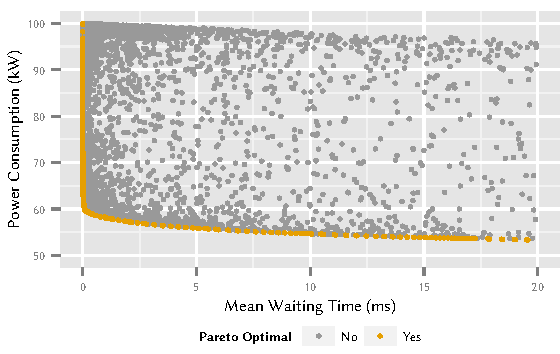
\includegraphics{cloud/data_centers/performance_evaluation/figures/energy_vs_waiting_pareto}
  \caption{Set of Pareto optimal values for the energy-efficient data centre.}
  \label{fig:cloud:data_centers:performance_evaluation:energy_vs_waiting_pareto}
\end{figure}

We plot all Pareto optima in \reffig{fig:cloud:data_centers:performance_evaluation:energy_vs_waiting_pareto}, the resulting curve has hyperbolic properties, going asymptotically to the mean waiting time \(E[W]\) as well as asymptotically to a parallel of the lower bound of the power drain \(E\).
This allows us to select an acceptable increase in mean waiting time \(E[W]\), for example one which would still satisfy a service level agreement, and harness the resulting energy savings.
On the other hand, we can decide on the required energy savings and infer if the corresponding mean waiting times are acceptable.
One possible parameter choice would allow the reduction of the power drain \(E\) by \SI{40}{\percent} while only increasing the waiting time by less then one millisecond.

\begin{figure}
  \centering
  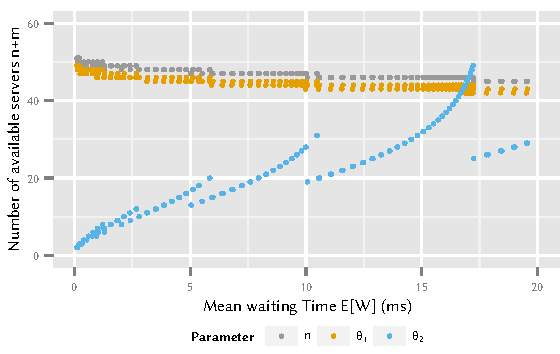
\includegraphics{cloud/data_centers/performance_evaluation/figures/sorted_results}
  \caption{Impact of parameter selection on mean waiting time \(E[W]\).}
  \label{fig:cloud:data_centers:performance_evaluation:sorted_results}
\end{figure}

Given the set of Pareto optima, we can investigate the parameter choice that leads to these optima.
To this end, we plot the system parameters for each optimum in \reffig{fig:cloud:data_centers:performance_evaluation:sorted_results}.
The optima themselves are sorted according to the mean waiting time \(E[W]\).
From the figure we observe see that generally, the server deactivation threshold is very close to the number of base-line servers, in most cases \(n - \theta_1 = 2\), the closest possible distance due to the macro state equation constraints.
Furthermore, the number of base-line servers is decreasing as the mean waiting time \(E[W]\) increases. 
The mean waiting time \(E[W]\) spectrum can be partitioned in interleaving sections, during which the number of base-line servers remain constant.
Furthermore, in such a section, the server activation threshold increases super linearly.
